\section{Implementation}
\label{sec:implementation}
The architecture discussed in Section~\ref{sec:arch} is implemented as a core
system, a user interface, and a set of modules. The system is written in Java.
\subsection{Core System}
\label{sec:core}
The core system is responsible for starting up the whole system. It first reads
the configuration file and establishes a connection with the data backend. The
core system is flexible as far as the backend is concerned and can communicate
with a variety of data backends including MySQL, Oracle, or flat files. The data
backend provides storage and lookup capabilities for user account informaton,
group information, access control information (as described in
Section~\ref{sec:access}), and component information. Once the connection to
the data backend has been established, the core system loads all the protocols,
devices, and applications modules in order. The core system contains an
Application Manager, Device Manager, and Protocol Manager to manage the various
types of components. It also keeps track of currently logged in users.
\subsection{Modules}
\label{sec:modules}
\begin{table}
\begin{center}
\begin{tabular}{| p{4cm} | p{3cm} |}
\hline
start() & Used by the Management Component to start the module \\ \hline
stop() & Used by the Management Component to stop the module \\ \hline
setModuleId() & Used by the Management Component to give the module an ID \\ \hline
getModuleId() & Used by the Management Component to get the ID of the module \\ \hline
getOfferedRoles() & Used by the Management Component to get the list of roles
offered by the module \\ \hline
serviceRegistered(roles) & Used by the Management Component to tell
the module that new roles are available \\ \hline
serviceDeRegistered(roles) & Used by the Management Component to tell
the module that some roles are no longer available \\ \hline
\end{tabular}
\end{center}
\caption{Module Interface}
\label{tab:module}
\end{table}

\begin{table}
\begin{center}
\begin{tabular}{| p{4cm} | p{3cm} |}
\hline
addModule() & adds a module to the system \\ \hline
removeModule() & removes a module from the system \\ \hline
getRole(String role) & Used by a module to request the ModuleManager to grant
access to a module offering the role sent as the parameter  \\ \hline
\end{tabular}
\end{center}
\caption{ModuleManager Interface}
\label{tab:modulemanager}
\end{table}
All applications, devices and protocols implement the Module interface. The
Module interface is required for a component to interact with the Management 
Component. Table~\ref{tab:module} provides an overview of the module interface.
Table~\ref{tab:modulemanager} provides an overview of the ModuleManager.
The ModuleManager is the part of the Management Component that interacts with
modules. Each module can offer some roles. Some modules might need specific
roles in order to fullfil their tasks. For example, an application (which is
also a module) that can turn on a light bulb would need a role called ``light
bulb.'' The application will ask the ModuleManager if there is a module that
offers the role ``light bulb.'' There can be another module, called
ZipatoLightBulb, that would be offering the role ``light bulb.'' If the
application has necessary permissions, the ModuleManger will allow the
application to interact with ZipatoLightBulb.
\subsection{User Interface}
\label{sec:interface}
\begin{figure}[tbh]                                                             
    \centering                                                                  
    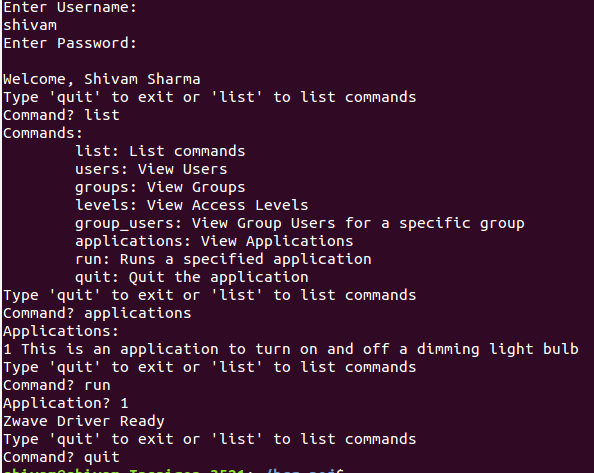
\includegraphics[width=1.0\columnwidth]{figs/cli.png}                
    \caption{Command Line Interface Screenshot}                                                      
    \label{Fig:cli}                                                            
\end{figure}
\begin{figure}[tbh]                                                             
    \centering                                                                  
    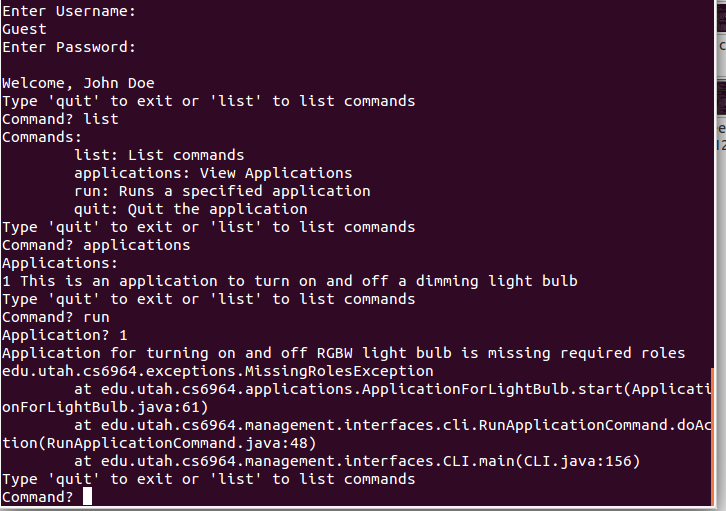
\includegraphics[width=1.0\columnwidth]{figs/cli2.png}                
    \caption{Command Line Interface Screenshot}                                                      
    \label{Fig:cli2}                                                            
\end{figure}
Currently, our system has a command line interface (CLI). We have designed the
user interface-related parts of our system in such a manner that replacing the
CLI with another interface in the future would be easily accomplished. The CLI
interacts with the core system to display information to the user and allow the
user to interact with the core system using a set of commands.

The CLI first asks the user to log in. Once the user has logged in, the CLI can
display a list of commands. The commands listed are based on the user's access
level (described in Section~\ref{sec:core_access}). Commands currently
implemented are: view users, view groups, view access levels, view users in
group, view applications, and run application.

Figure~\ref{Fig:cli} is a screenshot of the CLI for a user with access to all
commands. In the figure, after the user has logged in, he requests that the
system lists all commands available to him with the ``list'' command. Next, he
runs the ``applications'' command to view a list of currently available
applications (in this case our example application of turning a light bulb on
and off). Then, he runs our example application and quits. Whereas in
Figure~\ref{Fig:cli2} the user does not have permissions to view user and group
information. The user also does not have the permissions to run the example
application. Hence when the user tries to run it the system throws a
MissingRolesException.
\subsection{Access Control}
\label{sec:access}
Access control is divided into two types: core system access control and module
access control.
\subsubsection{Core System Access Control}
\label{sec:core_access}
The access control available for the core system (discussed in
Section~\ref{sec:core}) is designed to handle administrative tasks within the
core system. Users are divided into different levels of access. Currently, there
are eight levels of granularity, ranging from guests with minimal access to
full administrative users which have full permissions. Administrative tasks for
the core system include user account creation and modification, group creation
and assignment, and module access control administration.

Each user is assigned an access level, which is then used to determine which
commands the user can run. Each command is assigned a minimum access level.
When a user attempts to run the command, the access level of the user trying to
run the command is compared to the minimum access level of the command. If the
user's access level is greater than or equal to the minimum access level
assigned to the command, the user is able to run the command.
\subsubsection{Module Access Control}
Module access control provides access control between modules, which are
discussed in more detail in Section~\ref{sec:modules}. The access control
policies consist of a set of rules. Each rule consists of: a source module, a
destination module, the days of the week to which the rule applies, the start
and end times for those days, the user group to which the rule applies, the
priority of the rule, and the access mode.

When a user tries to use a module (either directly or indirectly), the system
looks for a rule that applies to the use. If a rule is found where the source
and destination modules match, then the system makes sure the current time and
day of the week match the rule and the user is part of the user group assigned
to the rule. The priority portion of the rule is used in the event of
conflicting access to the same module. The access mode can be either ``allow''
or ``ask.'' When the mode is ``allow,'' the interaction is automatically
allowed. When the mode is ``ask,'' a user is asked interactively to allow the
interaction at the time of access. Our system currently does not support the
priority or access mode portions of the rules.

Users are able to query the system to either figure out which modules a user can
access at a given time, based on the groups he or she is in, or figure out who
can access a given module. This allows the user to more reliably verify that the
access granted fits his or her expectations.
